%\documentclass[14pt, notes]{beamer}
\documentclass[14pt]{beamer}

%\usepackage{pgfpages}
%\setbeameroption{show notes}
%\setbeameroption{show notes on second screen=right}

%encoding
\usepackage[utf8]{inputenc}

%language
\usepackage[russian]{babel}
\usepackage{amsmath}
\usepackage{bm}
\usepackage{graphicx}
\usepackage{hyperref}
\usepackage{setspace}
\usepackage{tikz}
\usepackage{adjustbox}
\usepackage{marvosym}
\usetikzlibrary{shapes,arrows,positioning}
\makeatletter
%\@ifundefined{verbatim@out}{\newwrite\verbatim@out}{}
\makeatother
\graphicspath{{images/}}%путь к рисункам

\usepackage{tikz}
\usetikzlibrary{shapes,arrows}

\tikzstyle{decision} = [diamond, draw, fill=blue!20, text width=4.5em, text badly centered, node distance=3cm, inner sep=0pt]
\tikzstyle{block} = [rectangle, draw, fill=blue!20, text width=11em, text centered, rounded corners, minimum height=2em]
\tikzstyle{line} = [draw, -latex    ]
\tikzstyle{cloud} = [draw, ellipse,fill=red!20, node distance=3cm, minimum height=2em]

\setbeamerfont{author in head/foot}{size=\small}
\setbeamerfont{title in head/foot}{size=\footnotesize}
\setbeamercovered{invisible}
\setbeamertemplate{navigation symbols}{}%remove navigation symbols

\title[Моделирование движения жидкости в клапане]{Моделирование движения вязкой неоднородной жидкости в искусственном сердечном клапане}
\date{\today}
\author[Долгов Д.А.]{Долгов Д.А.\\ {\small аспирант кафедры вычислительной математики}\\ {\small Научный руководитель: Захаров Ю.Н.}}
\institute{Кемеровский Государственный Университет \\
    \vspace{0.7cm}
    \vspace{0.7cm}
} 
\usetheme[numbers, totalnumbers, minimal, nologo]{Statmod}
% Привычный шрифт для математических формул
\usefonttheme[onlymath]{serif}

\definecolor{statmodblue}{RGB}{100,10,30}
\definecolor{statmodsand}{RGB}{244,215,103}

\begin{document}
\maketitle

%description of the problem
\begin{frame}
\frametitle{Введение}
Искусственные клапаны являются эффективным способом лечения многих сердечно-сосудистых заболеваний. Их конструктивные особенности делают их одними из самых сложных медицинских устройств, используемых в кардиохирургии. Требования к функционированию клапанов очень велики - необходимо, чтобы он минимизировал турбулентность, создавал небольшой объем регургитации, позволял избегать зон застоя, разделения потока и т.д.
\end{frame}
\note{
    объем регургитации - объем обратного течения (из желудочка в атриум)
}

% valves placement
\begin{frame}
\frametitle{Схема расположения клапанов}
    \begin{center}
        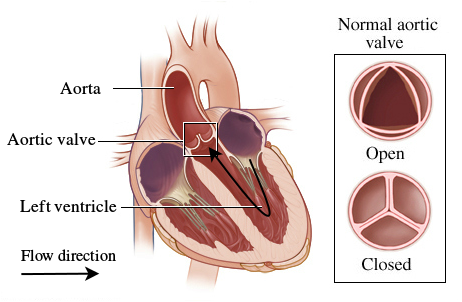
\includegraphics[width=8.5cm]{aorta_scheme.png}
    \end{center}
\end{frame}

% valve tissue structure
\begin{frame}
\frametitle{Схема строения тканей}
    \begin{center}
        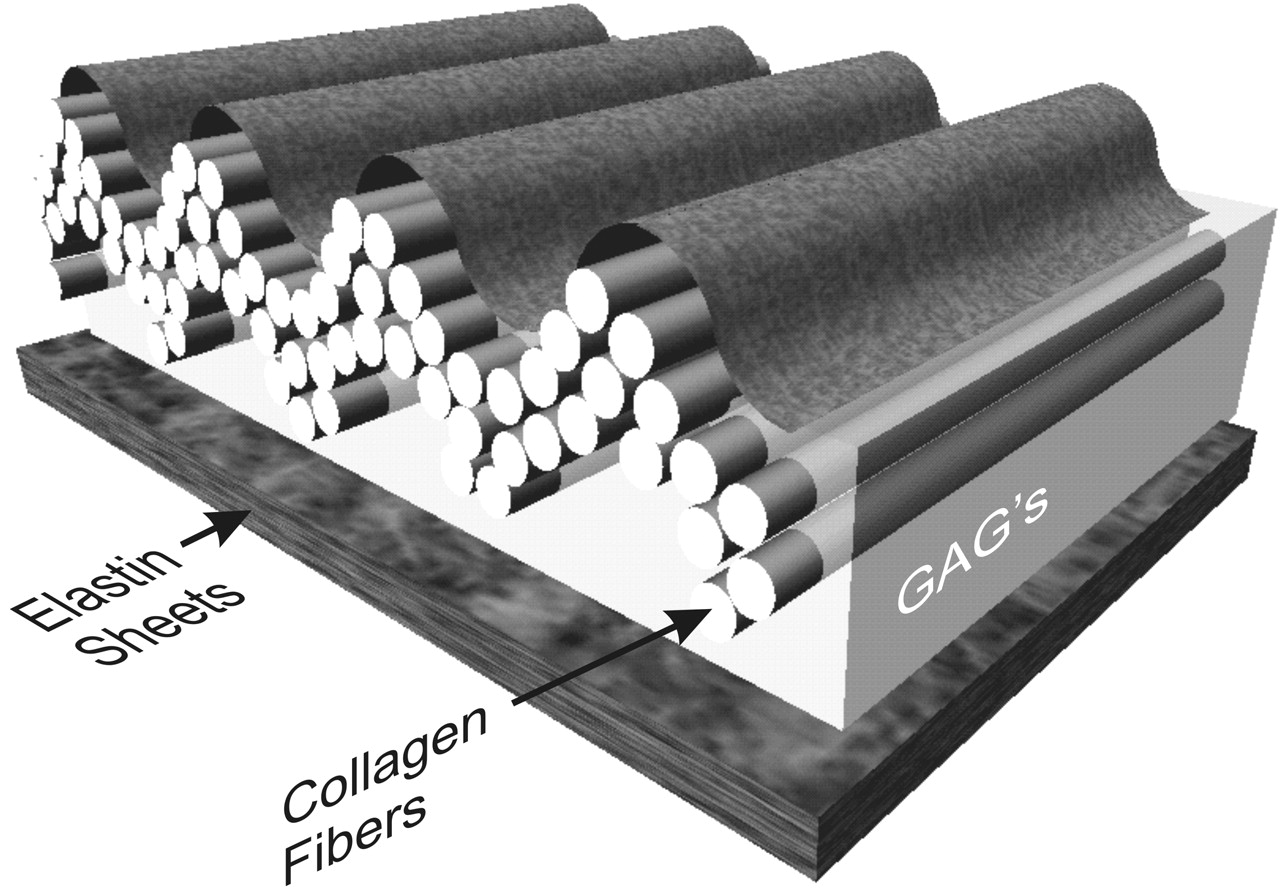
\includegraphics[width=8.5cm]{valve_tissue_structure.jpg}
    \end{center}

    \begin{spacing}{0.5}
        \mbox{\scriptsize
            Vesely, Ivan. "Heart valve tissue engineering." Circulation research 97.8 (2005): 743-755.
        }
    \end{spacing}

\end{frame}
\note{
    \begin{itemize}
        \item коллагеновые волокна (collagen fibers)
        \item слой эластина (белок) (elastin sheet)
        \item гликозаминогликаны (glycosaminoglycan matrix)
    \end{itemize}
}

% blood structure scheme
\begin{frame}
\frametitle{Схема структуры крови}
    \begin{center}
        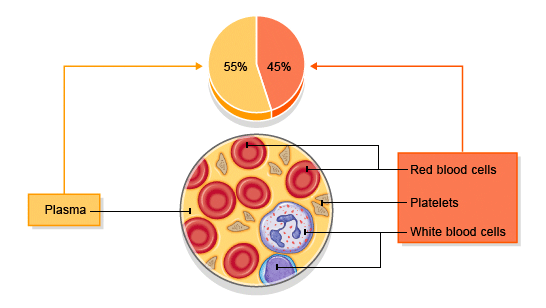
\includegraphics[width=8.5cm]{blood_scheme.png}
    \end{center}
\end{frame}

% papers overview
\begin{frame}
\frametitle{Обзор исследований}
    \begin{itemize}
        \item[\MVRightarrow] Kunzelman K.S., Reimink M.S. et al  Annular dilatation increases stress in the mitral valve and delays coaptation: a finite element computer model. (1997) Cardiovasc Surg 5(4):427–434
        \item[\MVRightarrow] Weinberg E. Dynamic simulation of heart mitral valve with transversely isotropic material model. Massachusetts Institute of Technology (2005)
        \item[\MVRightarrow] Kim H.S. Nonlinear multi-scale anisotropic material and structural models for prosthetic and native aortic heart valves. Georgia Institute of Technology (2009)
    \end{itemize}
\end{frame}
\note{
    Отметить, что рассматриваются работы, посвященные именно математическому моделированию клапанов,
    а не экспериментальному. На эту тему мало русскоязычных работ - даже в монографии "Искусственные клапаны сердца"
    (Орловский, Гриценко, Юхнев, Евдокимов, Гавриленков),
    где описан крупный вклад отечественных ученых в области клапанов, в разделе "Математическое моделирование" нет
    упоминаний о русскоязычных работах.
    Существует достаточно много (по крайней мере, зарубежных) исследований,
    посвященных математическому моделированию сердечных клапанов. В ранних моделируются
    только достаточно простые клапаны (по структуре, двумерные и проч.).
    Существует много современных работ, которые изучают клапан только с точки зрения
    эластичности, напряжений, возникающих при деформации и проч (при этом данные о давлении жидкости
    берутся либо из эксперимента, либо упрощенные, например течение Пуазеля).
    Самый перспективный вид исследований те, которые полноценно описывают взаимодействие потока и клапана,
    т.е. IBM
}

\begin{frame}
\frametitle{Обзор исследований}
    Расматривают только сам клапан и его деформации, представляя поток в упрощенном виде или
    вовсе получая данные о давлении экспериментально.
\end{frame}

% papers overview
\begin{frame}
\frametitle{Обзор исследований}
    \begin{itemize}
        \item[\MVRightarrow] Peskin, Charles S. "Numerical analysis of blood flow in the heart." Journal of computational physics 25.3 (1977): 220-252.
        \item[\MVRightarrow] Luo, X. Y., et al. "Effect of bending rigidity in a dynamic model of a polyurethane prosthetic mitral valve." Biomechanics and modeling in mechanobiology 11.6 (2012): 815-827.
        \item[\MVRightarrow] Flamini, Vittoria, Abe DeAnda, and Boyce E. Griffith. "Immersed boundary-finite element model of fluid-structure interaction in the aortic root." (2015).
    \end{itemize}
\end{frame}

\begin{frame}
\frametitle{Обзор исследований}
    Рассматривают полноценное взаимодействие ''жидкость-клапан'', позволяют считать клапан сколь угодно тонким.
    Не освещена тема потока жидкости с примесями.
\end{frame}

\begin{frame}
\frametitle{Описание модели}
Рассмотрим задачу о течении крови внутри крупных сосудов с гибкими стенками и клапаном. Кровь является неоднородной и состоит из плазмы и взвешенных в ней форменных элементов. Клапан и стенки сосуда являются гибкими и изменяют свою форму под воздействием течения. Будем моделировать кровь как вязкую, несжимаемую двухкомпонентную жидкость, а стенки сосуда - как поверхность заданной формы, обладающую определенной жесткостью.
\end{frame}

%description of the problem: schema
\begin{frame}
\frametitle{Описание модели}
    \begin{center}
        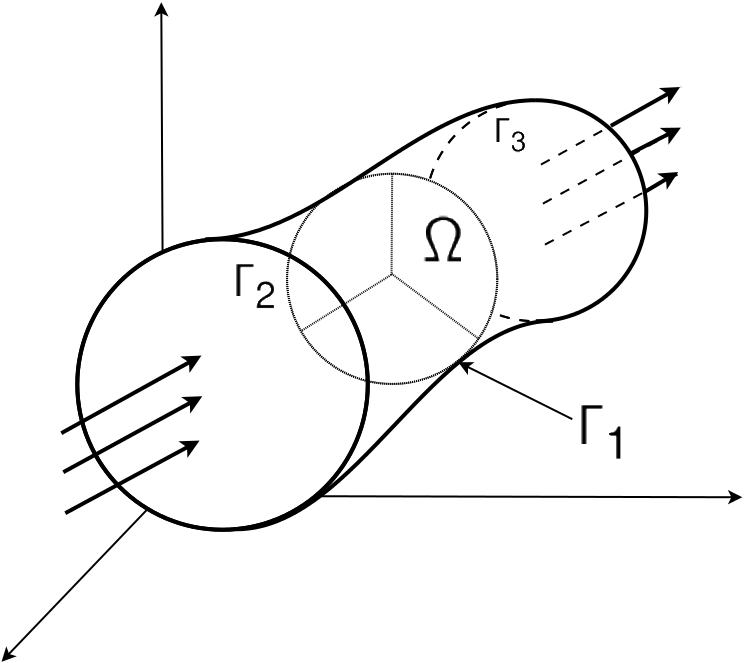
\includegraphics[width=8.5cm]{area_3d.png}
    \end{center}
\end{frame}
\note{$\Gamma_1$ - гибкие стенки, $\Gamma_2,\Gamma_3$ - вход/выход}

% navier stokes equations
\begin{frame}
\frametitle{Моделирование течения}
Система уравнений Навье-Стокса:
\begin{gather}
    \label{eq:motion}
    \frac{\partial u}{\partial t} + (u \cdot \nabla) u = - \frac{1}{\rho} \nabla p + \nabla \cdot \sigma + f\\
    \label{eq:continuity}
    \frac{\partial \rho}{\partial t} + \nabla \cdot (\rho u) = 0 
\end{gather}
где $\sigma = \mu (\nabla u + (\nabla u)^{T})$, $\bar{x} = (x, y, z) \in \Omega$ с начальными и краевыми условиями
\begin{gather*}
    u(\bar{x}, t_0) = u_0;\ \frac{\partial u}{\partial n}|_{\Gamma_2, \Gamma_3} = 0\\
    p|_{\Gamma_2} = p_{in};\ p|_{\Gamma_3} = p_{out} \\
\end{gather*}

\end{frame}
\note{Уравнения записаны в векторном виде, $\sigma$ - вязкий тензор напряжений}

% concentration
\begin{frame}
\frametitle{Концентрация}
Уравнение для расчета концентрации примеси в жидкости:
\begin{gather}
    \label{eq:concentration}
    \frac{\partial c}{\partial t} + u \cdot \nabla c = 0
\end{gather}
с начальными и краевыми условиями
\begin{gather*}
    c(\bar{x}, 0) = c_0(\bar{x})\\
    c(\bar{x}, t)|_{\Gamma_2} = c_s(\bar{x}, t)
\end{gather*}

\end{frame}

% concentration: dependencies
\begin{frame}
\frametitle{Концентрация}
Плотность и вязкость зависят от концентрации:
\begin{gather}
    \label{eq:concentration_viscosity}
    \mu = c (\mu_2 - \mu_1) + \mu_1\\
    \label{eq:concentration_density}
    \rho = c (\rho_2 - \rho_1) + \rho_1
\end{gather}

где $\mu_1, \mu_2, \rho_1, \rho_2$ - вязкости и плотности обоих компонент.
\end{frame}

% boundary
\begin{frame}
\frametitle{Сопротивление деформации}
В каждой точке сосуда и клапана определена поверхностная сила, которая стремится вернуть систему в равновесное положение
\begin{gather}
    \label{eq:strain_energy}
    F =  \frac{\partial}{\partial s}(T \tau) + \frac{\partial^2}{\partial s^2} \Big( E \cdot I \frac{\partial^2}{\partial s^2} X \Big)
\end{gather}
\begin{gather}
    \label{eq:define_boundary_force}
    F = k \cdot \|X - X_0\|
\end{gather}
\end{frame}
\note{$E$ - модуль Юнга, $I$ - момент инерции поперечного сечения, $T$ - напряжение фибры, $\tau$ - единичный тангенциальный вектор, касательный к фибре.}

% solve method 
\begin{frame}
\frametitle{Метод решения}
Будем рассматривать отдельно задачи вычисления параметров течения жидкости и параметров движения стенок сосуда и клапанов. Для этого введем в расчетной области сетки:
\begin{itemize}
    \item[\MVRightarrow] $\Omega_h = \Omega_h(x, y, z)$ - равномерная разнесенная сетка для расчета течения
    \item[\MVRightarrow] $\Gamma_h = \Gamma_h(q, r, s, t)$ - дополнительная сетка, соотнесенная со стенками сосуда и лепестками клапана (в лагранжевых координатах)
\end{itemize}

\end{frame}
\note{При обтекании жидкость какого-либо тела, она испытвает влияние силы давления рядом с границей тела (и сдвиговые силы, если есть условие прилипания). Исходя их этого обтекание тела можно моделировать с помощью поля внешних сил}

% solve method: diagram
\begin{frame}
\frametitle{Метод решения}
    \begin{center}
        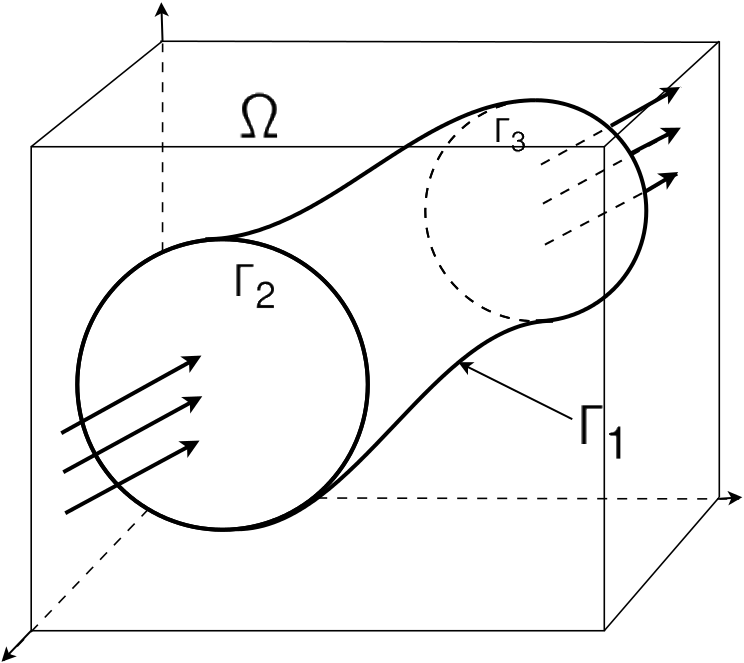
\includegraphics[width=8.5cm]{area_ibm_3d.png}
    \end{center}
\end{frame}

% solve method: diagram
\begin{frame}[fragile]
\frametitle{Алгоритм}
    \begin{adjustbox}{max totalsize={1.0\textwidth}{.7\textheight},center}
        \begin{tikzpicture}[node distance = 2.5cm, auto]
            \onslide<+->{
                \node[block]                           (init){
                    $u_0$, $p_0$, $\rho_0$, $\nu_0$
                };
            }

            \onslide<+->{
                \node[block, fill=none, minimum height=25em, text width=14em]          (fluid) at (6.8, -5){
                    $\Omega$
                };
                \node[block, right=1cm of init]            (body_forces_initial){
                    массовые силы $f_{ijk} = 0$
                };
                \path[line] (init) --                  (body_forces_initial);
            }

            \onslide<+->{
                \node[block, below of=body_forces_initial]            (navier_stokes){
                    уравнения Навье-Стокса
                };
                \path[line] (body_forces_initial) --                  (navier_stokes);
            }

            \onslide<+->{
                \node[block, below of=navier_stokes]   (concentration){
                    вычисление концентрации $c_{n+1}$
                };
                \path[line] (navier_stokes) --         (concentration);
            }

            \onslide<+->{
                \node[block, below of=concentration]   (viscosity_density){
                    вычисление $\nu_{n+1}$, $\rho_{n+1}$
                };
                \path[line] (concentration) --         (viscosity_density);
            }

            \onslide<+->{
                \node[block, below of=viscosity_density]   (new_flow){
                    $u_{n+1}$, $p_{n+1}$, $\rho_{n+1}$, $\nu_{n+1}$
                };
                \path[line] (viscosity_density) --     (new_flow);
            }

            \onslide<+->{
                \node[block, fill=none, minimum height=25em, text width=14em]          (fluid) at (14.8, -5){
                    $\Gamma$
                };
                \node[block, right= of new_flow, anchor=west](boundary_velocity){
                    перенос скорости жидкости на границу, $U_n$
                };
                \path[line] (new_flow) --         (boundary_velocity);
            }

            \onslide<+->{
                \node[block, right=of viscosity_density, anchor=west](deformation){
                    новая форма границы $X_{n+1}(X_{n}, U_{n}, t)$
                };
                \path[line] (boundary_velocity) --         (deformation);
            }

            \onslide<+->{
                \node[block, right=of concentration, anchor=west](boundary_forces){
                    сопротивление деформации $F_{n}(X_{n+1}, X_{n})$
                };
                \path[line] (deformation) --         (boundary_forces);
            }

            \onslide<+->{
                \node[block, right=of navier_stokes, anchor=west](body_forces){
                    новое распределение массовых сил $f_{ijk}$
                };
                \path[line] (boundary_forces) --         (body_forces);
                \path[line] (body_forces) --         (body_forces_initial);
            }

        \end{tikzpicture}
    \end{adjustbox}
\end{frame}

% solve method:split scheme
\begin{frame}
\frametitle{Алгоритм решения: поток}
Схема расщепления по физическим факторам:
\begin{gather}
    \label{eq:split_first}
    \frac{u^* - u^n}{\triangle t} = - (u^n \cdot \nabla) u^n + \frac{1}{\rho} \nabla \sigma + f\\
    \label{eq:split_second}
    \rho \triangle p^{n+1} - (\nabla p \cdot \nabla p^{n+1}) = \frac{\rho^2 \nabla u^*}{\triangle t}\\
    \label{eq:split_third}
    \frac{u^{n+1} - u^*}{\triangle t} = - \frac{1}{\rho} \nabla p^{n+1}
\end{gather}
где $\nabla \sigma (u^n, \mu) = \mu \triangle u^n + (\nabla \mu \cdot \nabla) u^n + (\nabla \mu \cdot J_{u^n}) $
\end{frame}
\note{
    \begin{itemize}
        \item[\MVRightarrow] Решаем уравнение \eqref{eq:split_first} методом стабилизирующей поправки (Дугласа-Рекфорда)
        \item[\MVRightarrow] Из уравнения \eqref{eq:split_second} методом бисопряженных градиентов определяем поле давления
        \item[\MVRightarrow] Восстанавливаем окончательное поле вектора скорости по явным формулам \eqref{eq:split_third}
    \end{itemize}
}

% solve method: boundary forces
\begin{frame}
\frametitle{Алгоритм решения: клапан}
\begin{gather}
    \label{eq:strain_energy}
    F_{n} =  \frac{\partial}{\partial s}(T_{n} \tau_{n}) + \frac{\partial^2}{\partial s^2} \Big( E \cdot I \frac{\partial^2}{\partial s^2} X_{n} \Big)
\end{gather}
\end{frame}
\note{$E$ - модуль Юнга, $I$ - момент инерции поперечного сечения, $T$ - напряжение фибры, $\tau$ - единичный тангенциальный вектор, касательный к фибре.}


% solve method:immersed boundary
\begin{frame}
\frametitle{Взаимодействие}
Уравнения, описывающие взаимодействие погруженной границы и жидкости:
\begin{gather}
    \label{eq:ibm_velocity}
    \frac{\partial X}{\partial t} = \int_{\Omega_h} u \cdot \delta (\bar{x} - X)\; dx\; dy\; dz \\
    \label{eq:ibm_force}
    f = \int_{\Gamma_h} F \cdot \delta (\bar{x} - X)\; dq\; dr\; ds\\
    \label{eq:no_slip}
    \frac{\partial X}{\partial t} (q, r, s, t) = u(X(q, r, s, t), t)
\end{gather}
\end{frame}
\note{Заглавные символы относятся к погруженной границе, обычные - к жидкости}

% solve method:ibm scheme
\begin{frame}
\frametitle{Взаимодействие}
Интерполяция скорости на погруженную границу и распределение силы сопротивления деформации:
\begin{gather}
    \label{eq:interpolation}
    U_n = \sum_{ijk}u_{ijk} \cdot D(x_{ijk} - x_n) h_{ijk}^3 \\
    \label{eq:spreading}
    f_{ijk} = \sum_n F_n \cdot D(x_{ijk} - x_n) h^2_n
\end{gather}

$D(x_n)$ соответствует $\delta(x - x_k)$.
\end{frame}

% solve method: force distribution scheme
\begin{frame}
\frametitle{Дельта-функция}
    \begin{center}
        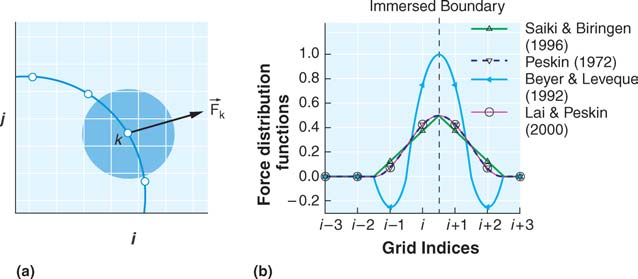
\includegraphics[width=11.5cm]{delta_function.png}
    \end{center}
\end{frame}

% totals and examples
\begin{frame}
\frametitle{Примеры}
    \begin{center}
        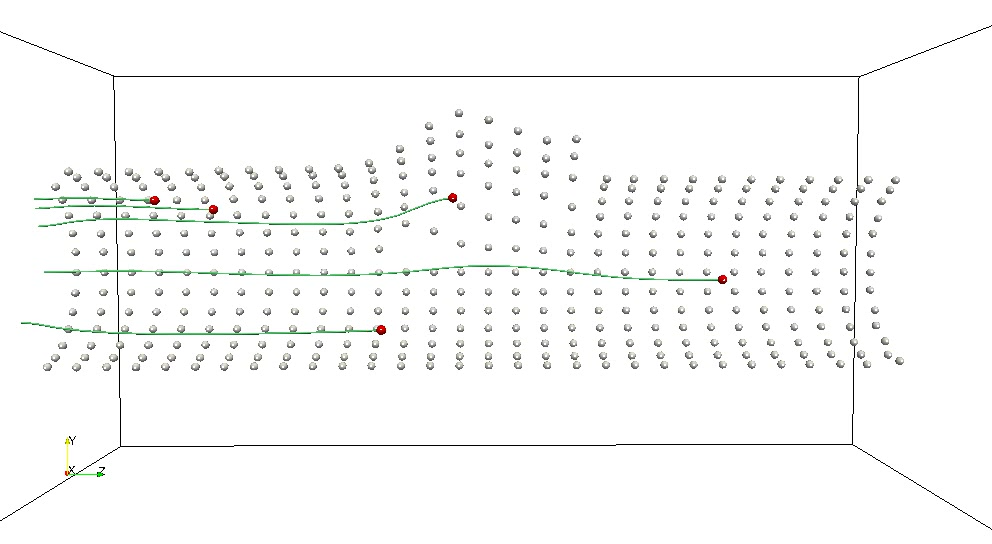
\includegraphics[width=5cm]{cylinder1_avi.png}
        \vspace{0.40mm}
        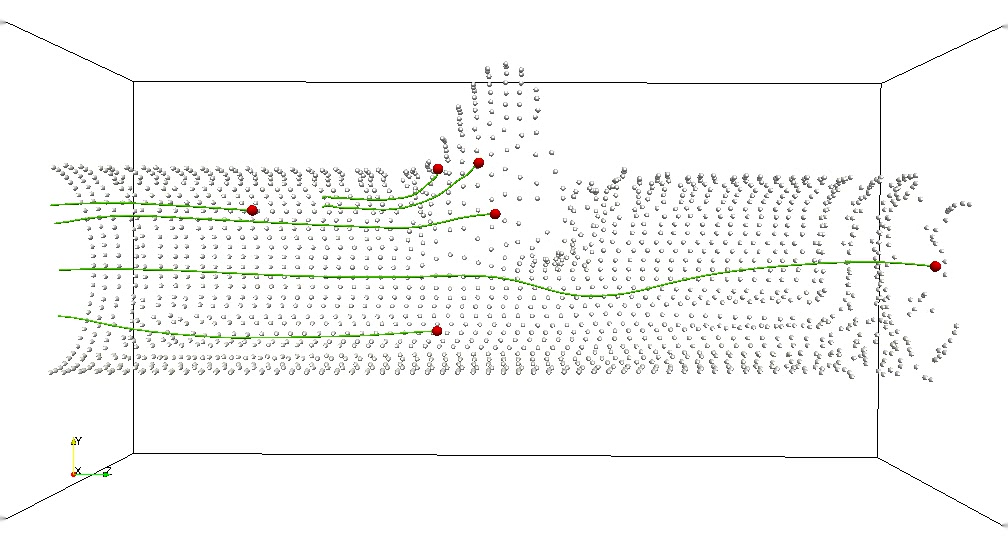
\includegraphics[width=5cm]{cylinder2_avi.png}
    \end{center}

\begin{itemize}
    \item[\MVRightarrow] \href{run:video/cylinder1.avi}{Деформация стенок сосуда}
    \item[\MVRightarrow] \href{run:video/cylinder2.avi}{Аналогичный расчет на более мелкой сетке}
\end{itemize}
\end{frame}

% totals and examples
\begin{frame}
\frametitle{Примеры}
    \begin{center}
        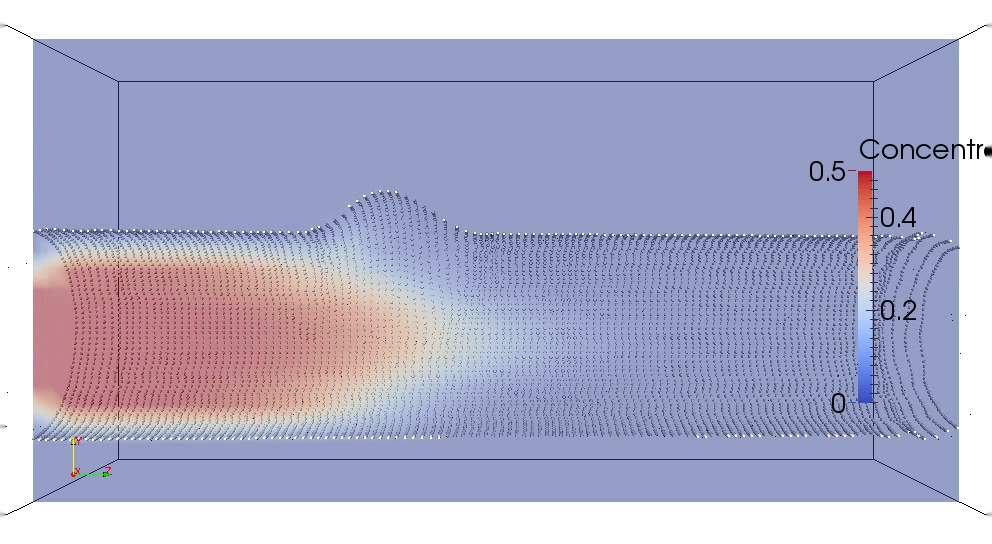
\includegraphics[width=5cm]{source_in_vessel_avi.png}
        \vspace{0.40mm}
        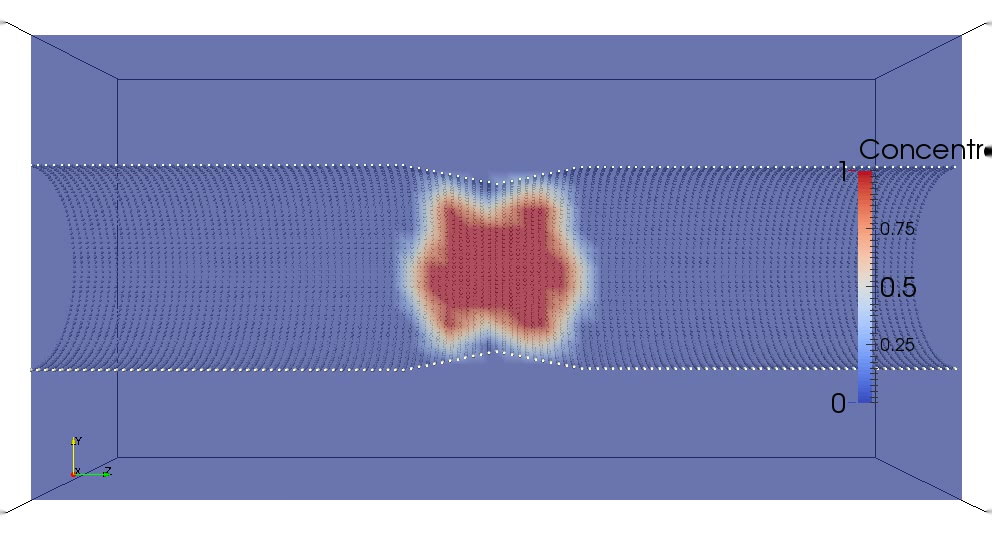
\includegraphics[width=5cm]{thrombus_in_vessel_avi.png}
    \end{center}

\begin{itemize}
    \item[\MVRightarrow] \href{run:video/source_in_vessel.avi}{Расчет распространения примеси}
    \item[\MVRightarrow] \href{run:video/thrombus_in_vessel.avi}{Размыв "тромба"}
\end{itemize}
\end{frame}

\begin{frame}
\frametitle{Примеры}
    \begin{center}
        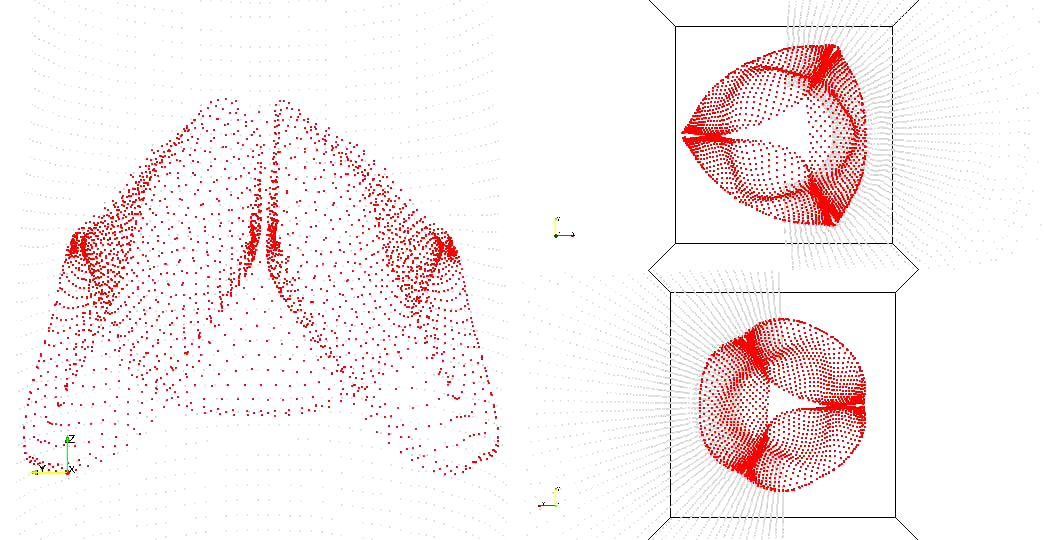
\includegraphics[width=5cm]{valves_closing_accurate_two_avi.png}
        \vspace{0.40mm}
        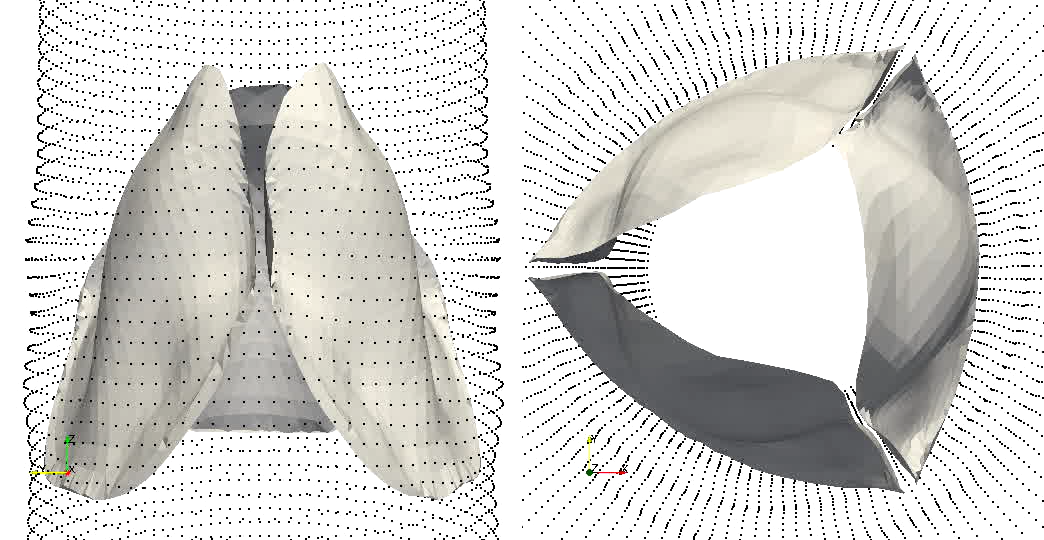
\includegraphics[width=5cm]{valve_delaunay.png}
    \end{center}

\begin{itemize}
    \item[\MVRightarrow] \href{run:video/valves_closing_accurate_two.avi}{Движение клапана}
    \item[\MVRightarrow] \href{run:video/valve_delaunay.avi}{Движение клапана (поверхность)}
\end{itemize}
\end{frame}

\begin{frame}
\frametitle{Примеры}
    \begin{center}
        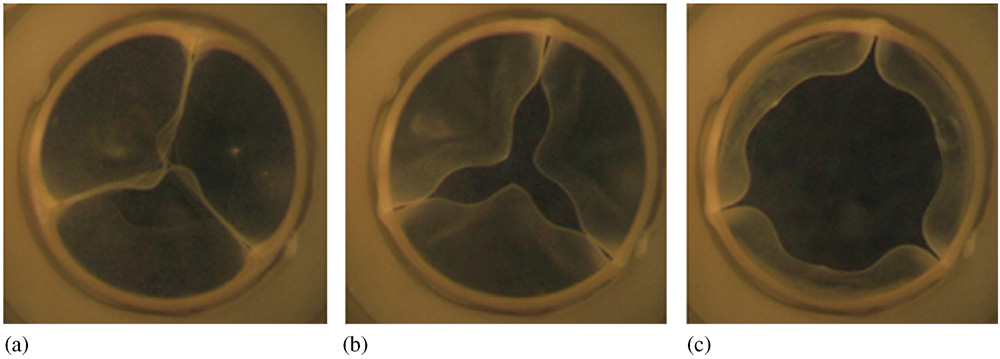
\includegraphics[width=11cm]{aortic_valves.jpg}
    \end{center}

\begin{spacing}{0.5}
{\scriptsize
    Watton PN, Luo XY et al (2007) Dynamic modelling of prosthetic
    chorded mitral valves using the immersed boundary method.
    J Biomech 40(3):613–626 Watton PN, Luo XY et al (2008) Effect of ventricle motion on the
}
\end{spacing}

\end{frame}

\begin{frame}
\frametitle{График расхода жидкости}
    \begin{center}
        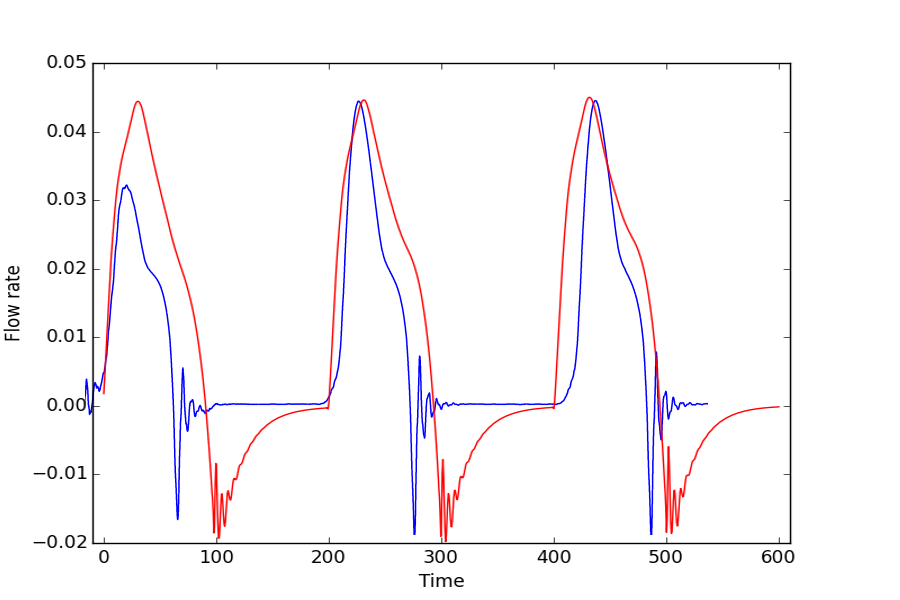
\includegraphics[width=10cm]{flow_rate_comparison.png}
    \end{center}

    \begin{adjustbox}{max totalsize={1.0\textwidth}{.7\textheight},center}
        {\scriptsize
            International Journal for Numerical Methods in Biomedical Engineering 28.3 (2012): 317-345.
            %"Immersed boundary model of aortic heart valve dynamics with physiological driving and loading conditions." International Journal for Numerical Methods in Biomedical Engineering 28.3 (2012): 317-345.
        }
    \end{adjustbox}
\end{frame}
\end{document}
